\newcommand{\figuraPresionTierra}{%
\begin{figure}[H]
    \centering
    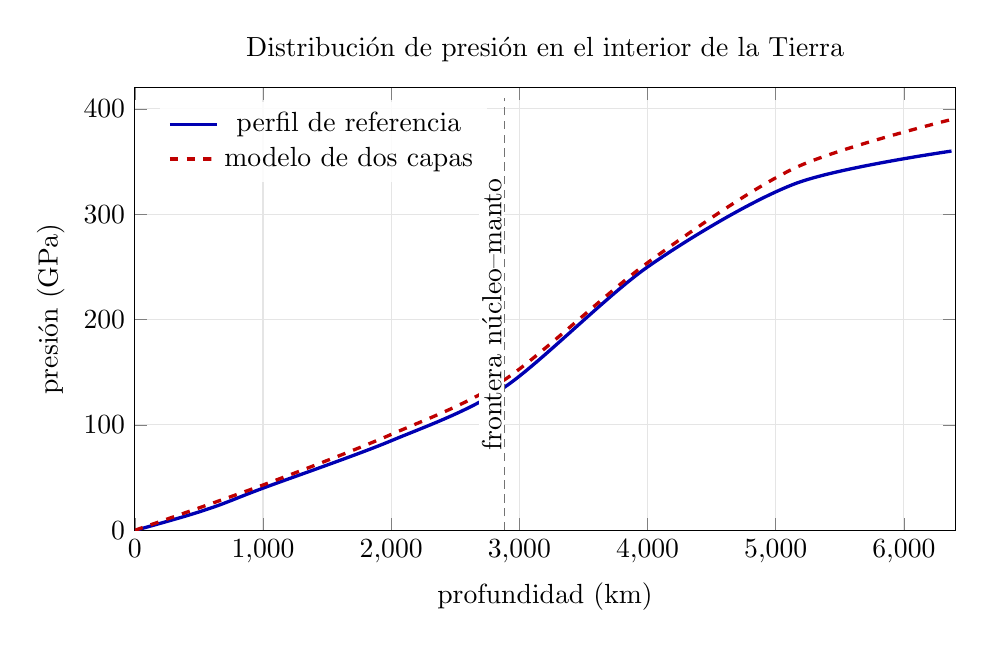
\begin{tikzpicture}
        \begin{axis}[
            width=12cm,
            height=7.2cm,
            xmin=0,xmax=6400,
            ymin=0,ymax=420,
            xlabel={profundidad (km)},
            ylabel={presión (GPa)},
            title={Distribución de presión en el interior de la Tierra},
            grid=major,
            grid style={gray!20},
            legend style={at={(0.03,0.97)},anchor=north west,
                          draw=none,fill=white,fill opacity=0.85,
                          text opacity=1}]

            \addplot[very thick,blue!70!black,smooth]
                coordinates {
                    (0,0) (35,1) (410,14) (660,24) (1000,40)
                    (2000,85) (2886,136) (4000,250)
                    (5150,329) (6371,360)
                };
            \addlegendentry{perfil de referencia}

            \addplot[very thick,red!75!black,dashed,smooth]
                coordinates {
                    (0,0) (1000,43) (2000,91) (2886,143)
                    (4000,254) (5150,344) (6371,390)
                };
            \addlegendentry{modelo de dos capas}

            \draw[densely dashed,black!55]
                (axis cs:2886,0)--(axis cs:2886,410);
            \node[rotate=90,anchor=south,fill=white,inner sep=1pt]
                at (axis cs:2886,205) {frontera núcleo--manto};
        \end{axis}
    \end{tikzpicture}
    \caption{Comparación cualitativa entre un perfil terrestre de referencia
    y el modelo de dos capas con densidades constantes. El modelo elemental
    reproduce la escala de la presión central y el cambio de pendiente en la
    frontera núcleo--manto.}
    \label{fig:presion-tierra}
\end{figure}%
}